\chapter{Cronograma de execução do projeto}

Como ilustra a seta em amarelo na Fig. \ref{crono}, este projeto terá a duração de um ano com início em 2021 e término em 2022, e estará focada no desenvolvimento do sensor LGAD e na construção e teste do protótipo do HGTD. 

O plano de execução para o desenvolvimento do LGAD, mostrado na Fig. \ref{crono}, tem a duração total de cinco anos (2020 - 2025), onde estão inclusas as fases de desenvolvimento do sensor - início de 2020 até o início de 2022 - e produção dos dispositivos LGAD, de 2022 até 2024. 
\thispagestyle{plain}

Além das atividades de desenvolvimento do LGAD, durante este período o cronograma também prevê a construção do HGTD (\textit{demonstrator}), e a sua caracterização com raios cósmicos e raios-X. Essas duas fases são importantes pois permitirão o desenvolvimento das atividades relacionadas com a construção do HGTD, a caracterização de seus diversos componentes, bem como a sua integração com a eletrônica de aquisição de dados, corroborando com os objetivos propostos neste documento. 

\begin{figure}[H]
    \centering 
    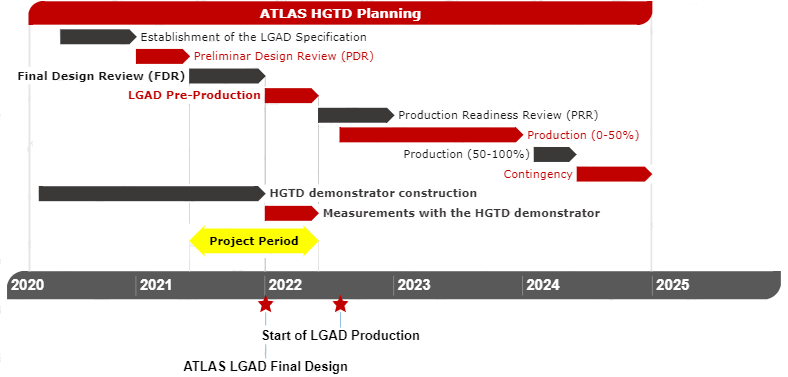
\includegraphics[width=16.0cm]{assets/cronogama.png}
    \caption{Figura mostrando o planejamento para o desenvolvimento do LGAD e HGTD, incluindo as revisões do projeto (PDR, FDR, PRR), pré-produção e produção. Os principais {\it milestones} do projeto são mostrados em sua linha do tempo.}
    \label{crono}
\end{figure}

\renewcommand{\cleardoublepage}{}
\renewcommand{\clearpage}{}